% Document template suitable for use as a LaTeX master-file 
% for thesis works in University of Turku Department of Computing
%
% Technical usage guide: https://tech.utugit.fi/soft/thesis/doc/doc/overview/
% 

\documentclass[language=english,version=final,mainfont=none,sharelatex=true,minted=true]{utuftthesis}
\setcounter{secnumdepth}{2}
\setcounter{tocdepth}{2}
\usepackage{float}
\usepackage[caption=false]{subfig}
\usepackage{enumitem}

% Define the algorithm environment
%\makeatletter
\providecommand\textquotedblplain{%
  \bgroup\addfontfeatures{Mapping=}\char34\egroup}
\providecommand{\tabularnewline}{\\}
\floatstyle{ruled}
\newfloat{algorithm}{tbp}{loa}
\providecommand{\algorithmname}{Algoritmi}
\floatname{algorithm}{\protect\algorithmname}
%\makeatother

\addbibresource{Bibliografia.bib}

\begin{document}

\pubyear{2023}
\pubmonth{6}
\publab{Tietojenkäsittelytiede}
\publaben{Computer Science}
\pubtype{gradu}
\title{Trusted Execution Environments in Protecting Machine Learning Models}
\author{Maks Turtiainen}

\newlist{questions}{enumerate}{2}
\setlist[questions,1]{label=\textbf{RQ\arabic*.},ref=RQ\arabic*}
\setlist[questions,2]{label=(\alph*),ref=\thequestionsi(\alph*)}

\maketitle

\keywords{Trusted Execution Environment, TEE, Software Guard Extension, Intel SGX, Machine Learning, Gramine}

\begin{abstract}
The adaptation and application of machine learning (ML) has grown extensively in recent years, and has awakened concern about the safety of intellectual property (IP) related to the machine learning models. The training of machine learning models is a time-consuming and expensive task, that has increased the demand of better solutions to protect the intellectual property of the machine learning models. This thesis explores the promising potential of Trusted Execution Environments (TEE) like Intel's Software Guard Extensions (Intel SGX), in protecting intellectual property related to machine learning models. The concern of ML model safety arises especially when the software solution needs to be distributed to clients or machine learning operations needs to be done in an untrusted environment. The main focus of this thesis is on Intel's SGX, which is one of the most used TEE implementations. This thesis tries to answer to the questions on how TEEs can be used to protect IP of the ML models, what aspects need to be considered and what limitations may arise.
\end{abstract}

% mandatory
\tableofcontents

% if you want a list of figures
\listoffigures

% if you want a list of tables
\listoftables

% if you want a list of acronyms
%\listofacronyms

% change the name if the default doesn't sound right
\renewcommand{\algorithmname}{\listingscaption}

% The thesis starts here.

\chapter{Introduction} \label{Introduction}

In recent years, machine learning (ML) has witnessed an unprecedented increase in its adoption across various domains, ranging from finance and healthcare to autonomous vehicles and natural language processing. As the ML models can have remarkable ability to learn and make predictions from vast amounts of data and the training of these ML models can be expensive and time-consuming, the ML models have become valuable assets for companies. However, with the increasing adoption of machine learning models comes the concern of protecting the intellectual property (IP) associated with these ML models.

Trusted Execution Environments (TEEs) have emerged as a promising solution to address the challenges associated with IP protection of machine learning models. TEEs provide a secure and isolated environment where sensitive computations, such as those involved in using and training machine learning models, can be executed securely, protecting the confidentiality and integrity of the underlying algorithms and data.

The most significant concern that arises is the risk of model theft or unauthorized replication of the machine learning models. The concern arises mainly when ML application needs to be run in an untrusted environment. The untrusted environment can be, for example, an infrastructure of a customer to whom the machine learning application is distributed. Untrusted environment can also be third-party cloud infrastructure. Unauthorized access to the ML models can lead to their replication, reverse engineering, or even the extraction of sensitive information embedded within them.\cite{ipofml}

Trusted Execution Environments offer a solution to address these concerns. By using hardware-based security technologies, such as Intel SGX (Software Guard Extensions), AMD SEV (Secure Encrypted Virtualization) and ARM TrustZone, TEEs create a secure and isolated enclave where sensitive computations can be isolated from the rest of the system. Isolation ensures that even privileged software cannot access or tamper with the sensitive data and algorithms processed inside the enclave.\cite{teeieee}

This thesis explores the potential of TEEs in protecting Intellectual Property associated with machine learning models when the machine learning application needs to be distributed to the client with the ML model bundled within it. Trusted Execution Environment implementation chosen for closer examination is Intel SGX. This thesis tries to answer to the questions on how Intel SGX can be used to protect the IP of the ML models, what aspects need to be considered and what are the limitations, from the perspective of ML model Intellectual Property protection. Application of Intel SGX is explored and existing techniques and frameworks are discussed. This thesis also provides an example implementation of a machine learning application that uses Intel SGX to protect the IP of the ML model. The research questions of this thesis can therefore be formulated as follows:

\begin{questions}[itemindent=2em]
        \item\emph{What is currently known about different TEE implementations and their potential in protecting IP associated with ML models?\label{rq1}}
        \item\emph{How TEEs, especially Intel SGX, can be used to protect the IP associated with ML models when ML application is distributed to end-users?\label{rq2}}
        \item\emph{What issues and limitations should be considered when applying TEEs, especially Intel SGX, for IP protection associated with ML models?\label{rq3}}
\end{questions}

Chapter \ref{problem} discusses the concerns raised in more detail. Even though this thesis focuses on the problem when ML application is distributed with ML model, the scenario when ML application runs inside untrusted cloud infrastructure is briefly discussed. Although this specific topic has not been previously researched, Chapter \ref{prev-res} explores the previous research around this topic. Chapter \ref{ml} gives a brief introduction to the machine learning and explores different types of machine learning and current popular techniques to implement them. Chapter \ref{tees} presents Trusted Execution Environments and the most common use cases of them. Different TEE implementations are introduced, with the focus on Intel SGX, which is discussed in more detail. Chapter \ref{solution} offers a practical solution to the concerns of ML model IP protection. The example implementation that is made as a part of this thesis is presented in this chapter. To practically demonstrate the limitations of Intel SGX, the example implementation is used to conduct performance testing. The results of the performance testing are also presented in this chapter. Chapter \ref{conclusion} concludes this thesis by pulling together the main findings.

\chapter{The Problem} \label{problem}

As the training of the machine learning model is time-consuming and requires plenty of export effort, it is usually expensive. Due to the expensive nature of ML model training, it is often desired to protect the Intellectual Property of the ML model. Whether the intellectual property of the ML model is safe arises in multiple different scenarios, the most obvious being that when a software solution containing the ML model is distributed to the end-user.

Next, the two most typical scenarios where the IP of the ML model can become compromised are discussed.

\section{Problem When Distributing Software} \label{problem-dist}

In some cases, software solutions that contain machine learning computations are separated into the client part and the server part. By separating software solutions into client and server, only the client part needs to be distributed to the end-user and the software distributor can provide access to the server part of the software which contains the machine learning models. The server part is then run inside the software distributor's own trusted infrastructure, and the intellectual property of the ML model can be considered safe. However, Canadian research from last year suggests that the ML model can still be stolen through API extraction\cite{difficulty}.

But in other cases, the machine learning application needs to be distributed in its entirety to the end-users, including machine learning models. This is the case, especially when the machine learning application cannot rely on a stable internet connection to query the machine learning application server, for example in self-driving solutions in cars and marine vessels. Protecting intellectual property of the ML model in this scenario is in the main focus of this thesis.

Without any protection, this practice exposes ML models to potential threats that can compromise the intellectual property of these models. 

ML models embedded within applications can be reverse engineered by attackers, allowing them to extract the underlying algorithms, model architecture, or even training data. This process enables potential competitors or malicious actors to replicate or modify the model without permission, posing a significant threat to the original model's intellectual property.

\section{Problem When Using Cloud Environments} \label{problem-cloud}

As cloud computing services are very popular, they should be briefly discussed, even though the focus of this thesis is on the case when ML application is distributed entirely to the end-users. Cloud computing services raise concern whether the third-party cloud infrastructure providers can be completely trusted. This question has been investigated in many contexts, as the most popular cloud infrastructure provider companies are from the United States. Many European Union countries have policies not to use third-party cloud infrastructure when public sector application can process sensitive information.

\section{Limitations of Existing Approaches} \label{limit}

There are techniques designed to protect the IP any data like data obfuscation, but none of them provides complete solution to the problem.

\subsubsection{Data Obfuscation} \label{obfuscation}

Commonly employed techniques, such as obfuscation, aim to hinder reverse engineering by transforming the ML model's code or structure. However, these methods often fall short, as skilled attackers can still reverse engineer the transformed models, posing a significant risk to the intellectual property of the ML model.\cite{obfuscation}

\subsubsection{Legal Protection} \label{legal}

While legal frameworks exist to protect intellectual property, enforcing them in the context of ML models can be challenging. Copyright and patent laws may not adequately address the unique challenges presented by the machine learning models. Furthermore, legislations are different in different countries and there are parties that do not care about legal sanctions.

\chapter{Previous Research} \label{prev-res}

The subject of using Trusted Execution Environments to protect IP of ML models has been researched a little in the past. This chapter partly answers to the \ref{rq1}.

There are at least three papers published specifically on the subject; \textit{SecureTF: A Secure TensorFlow Framework (2020)}\cite{securetf}, \textit{Using Intel SGX to Improve Private Neural Network Training and Inference (2020)}\cite{usingsgx} and \textit{Securely Exposing Machine Learning Models to Web Clients using Intel SGX (2019)\cite{securely}}. However, none of these papers discusses specifically the problem when the ML application is distributed entirely to the end-users.

This chapter also mentions two other studies which are related, but whose objectives did not include protection of machine learning models. Gramine Project\cite{gramine}, which includes two papers and framework software, is mentioned first and then paper \textit{SGXCrypter: IP protection for portable executables using Intel's SGX technology (2017)}\cite{sgxcrypter}. Although their goal is not specifically to protect machine learning models, they still can be considered relevant.

\subsubsection{SecureTF: A Secure TensorFlow Framework} \label{securetfa}

\textit{SecureTF: A Secure TensorFlow Framework} by Roland Kunkel, Franz Gregor and Do Le Quoc from TU Dresden, Sergei Arnautov and Christof Fetzer from Scontain UG and Pramod Bhatotia from University of Edinburgh provides a complete, ready-to-use framework to use a popular and open-source machine learning and artificial intelligence library TensorFlow securely with Trusted Execution Environments. Because the machine learning operations require a lot of computation power, the machine learning operations are often done on third-party cloud infrastructure.

The main concern of the writers of this paper was how to do machine learning operations securely in the untrusted cloud environment. The paper investigates the training phase as well as the classification phase of the machine learning process. In the training phase, the datasets used to train the model can be considered information that must be protected. On the other hand, in the classification phase, the model itself becomes valuable intellectual property and can be considered information that must be protected.

As a solution to this concern, the writers of this paper propose SecureTF, a framework which bundles the machine learning application with all needed libraries into a software that is transferred to the TEE enclave in its entirety. Machine learning models and training data provided to the enclave encrypted, which are then decrypted inside the enclave after successful remote attestation. The high-level system overview can be seen in Figure \ref{img:securetf}.

\begin{figure}
\centering 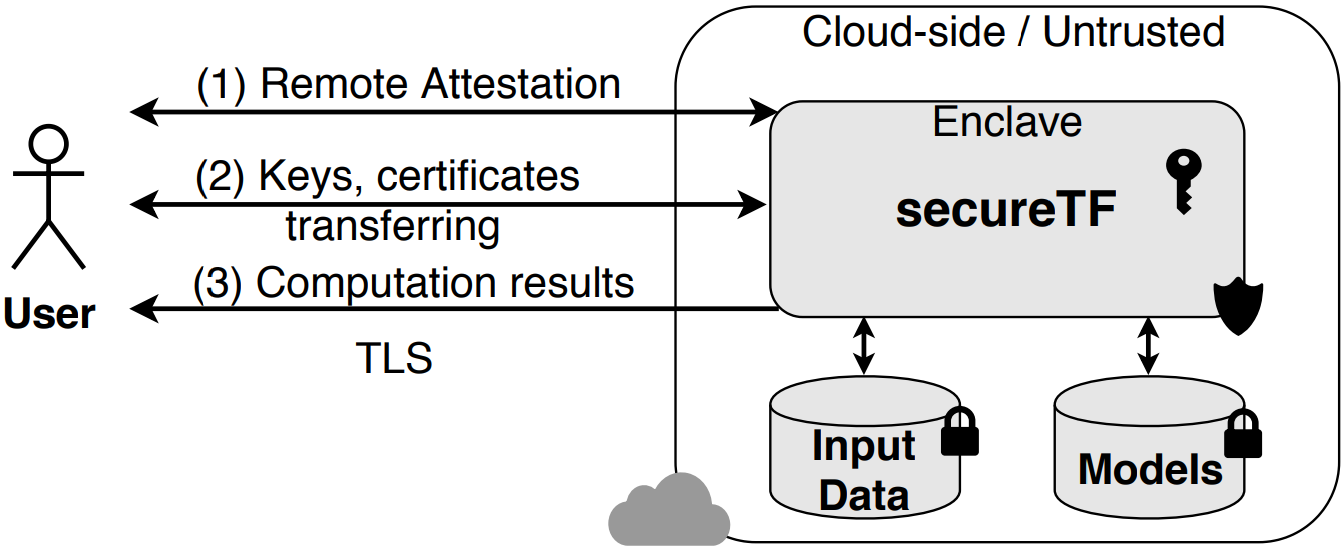
\includegraphics[width=0.7\textwidth]{img/securetf}
\caption{System overview of SecureTF from \textit{SecureTF: A Secure TensorFlow Framework}}
\label{img:securetf} 
\end{figure}

The same authors also earlier wrote \textit{TensorSCONE: A Secure TensorFlow Framework using Intel SGX}\cite{tensorscone} that is focused on the same concerns, but the implementation was specifically done for Intel SGX.

\subsubsection{Using Intel SGX to Improve Private Neural Network Training and Inference} \label{improveprivate}

\textit{Using Intel SGX to Improve Private Neural Network Training and Inference} by Ryan Karl, Jonathan Takeshita and Taeho Jung from University of Notre Dame is a bit shorter paper where the main focus is on the running the inference phase of the Deep Neural Network (DNN) machine learning algorithm in an untrusted cloud infrastructure.

The approach is more theoretical and proposes a mathematical method which includes encrypting to run machine learning inference securely in an untrusted environment. There is no implementation discussed.

\subsubsection{Securely Exposing Machine Learning Models to Web Clients using Intel SGX} \label{securelyexposingml}
 
\textit{Securely Exposing Machine Learning Models to Web Clients using Intel SGX} by Dávid Ács and Adrian Coleşa from Technical University of Cluj-Napoca discusses the possibility to serve the machine learning model as a part of a web application, but still keeping it secure. Their main concern is that even though the server infrastructure could be considered secure, there might be latency and performance loss when the machine learning application is used through the internet, in a web application.

The method proposed in this paper is to serve the machine learning application and related models to the client's web browser. The web browser initializes an Intel SGX enclave, where the confidential data can be processed securely, without exposing them outside the enclave. The proposed method includes a web page, browser extension, native client-side application, server and usage of Intel's Remote Attestation. The client must fully support Intel SGX. The architecture overview can be seen in Figure \ref{img:websgx}.

\begin{figure}
\centering 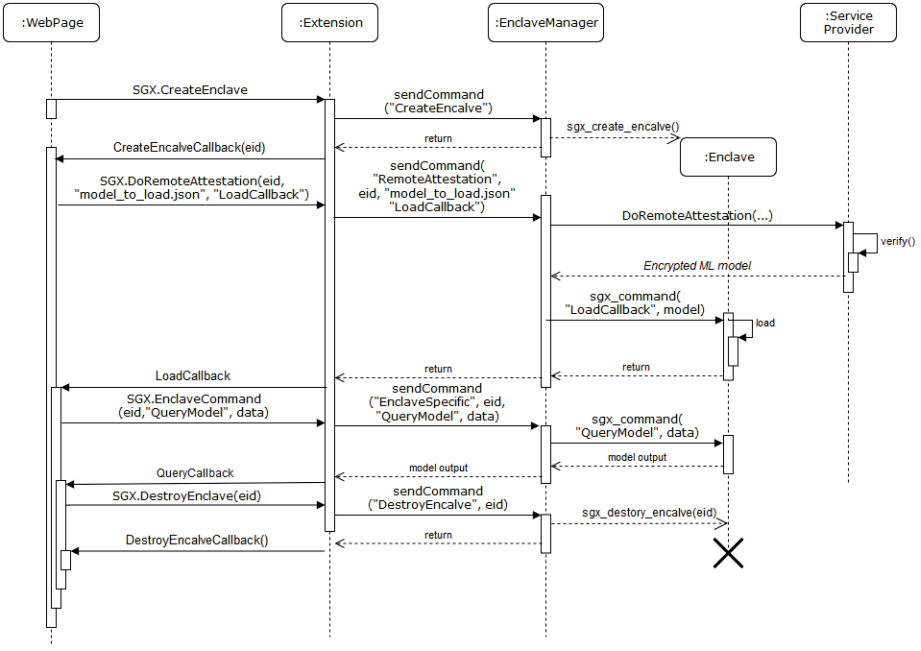
\includegraphics[width=0.8\textwidth]{img/websgx}
\caption{Query and load sequence diagram of proposed method from \textit{Securely Exposing Machine Learning Models to Web Clients using Intel SGX}}
\label{img:websgx} 
\end{figure}

\subsubsection{Gramine Project} \label{prevgramine}

Gramine Project, originally launched by OSCAR LAB at Stony Brook University, has become an important part of this thesis. Gramine, which was originally called Graphene, is a library operating system (LibOS) with Intel SGX support which is perfectly suitable for protecting intellectual property of ML models. Gramine will be discussed in detail in Section \ref{gramine}.

Gramine team has published two papers regarding their project; \textit{Cooperation and Security Isolation of Library OSes for Multi-Process Applications (2014)}\cite{graminepaper} and \textit{Graphene-SGX: A Practical Library {OS} for Unmodified Applications on SGX (2017)}\cite{graminesgxwp}.

\begin{figure}
\centering 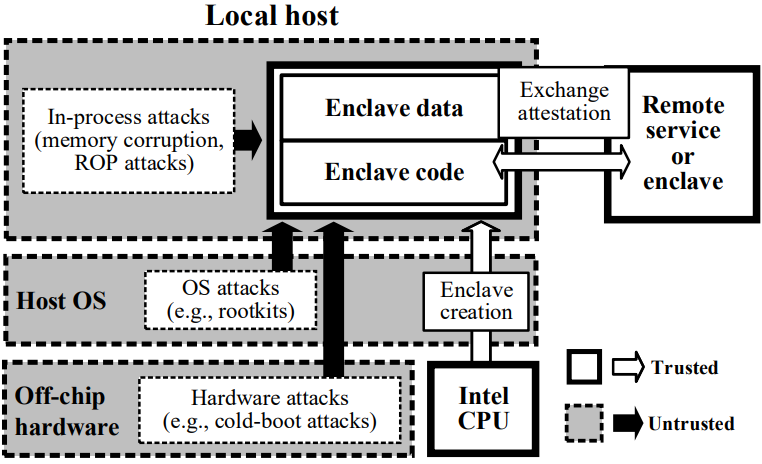
\includegraphics[width=0.7\textwidth]{img/graminethreat}
\caption{The threat model of SGX, presented in \textit{Graphene-SGX: A Practical Library {OS} for Unmodified Applications on SGX}. Intel SGX protects applications from three types of attacks: in-process attacks from outside the enclave, attacks from the OS or hypervisor, and attacks from off-chip hardware.}
\label{img:threatmodel} 
\end{figure}

\subsubsection{SGXCrypter: IP protection for portable executables using Intel's SGX technology} \label{sgxcrypter}

One research that can be considered relevant from the perspective of protecting machine learning models is \textit{SGXCrypter: IP protection for portable executables using Intel's SGX technology} by Dimitrios Tychalas and Michail Maniatakos from New York University Abu Dhabi and Nektarios Georgios Tsoutsos from NYU Tandon School of Engineering. The main concern of this study was the compromised intellectual property through reverse engineering. The existing techniques to make reverse engineering impossible, such as data obfuscation, have been found unsuitable, especially because data obfuscation is a common technique used by malware authors. Antivirus engines often consider executables with obfuscated data as a malicious software.

The paper proposes a special encryption schema to encrypt Microsoft Windows software executables. Windows software executables have an encrypted payload section that can be decrypted by the client's Trusted Execution Environment -- Intel SGX enclave. By using this approach, anything inside the executables encrypted payload, for example a machine learning model, is never exposed to the other parts of the client's system.
\chapter{Machine Learning} \label{ml}

Machine Learning (ML) is a subfield of Artificial Intelligence (AI). AI is not strictly defined, as the Intelligence itself is not strictly defined. The strict definition of these terms tends to drift more to the field of philosophy than to the field of computer science.\cite{wang2019defining}

Simply put, machine learning is a method to learn to do certain tasks based on data. Machine learning algorithms build models by recognizing and extracting patterns from given training data. Machine learning can be divided into three main types; Supervised Machine Learning, Unsupervised Machine Learning and Reinforcement Learning. Deep learning can be seen as a fourth type of machine learning, that can use techniques from other types of machine learning.\cite{alpaydin2020introduction}

A machine learning model is a mathematical function that is created through the process of training a machine learning algorithm on a given dataset. It captures patterns, relationships, or dependencies in the data and is used for making decisions, predictions, classifications, or other ML operations. ML model can be seen as a `learned' version of the ML algorithm that can generalize from the training data to make predictions or decisions on new, similar data.

\section{Introduction to Artificial Intelligence} \label{ai}

One common and perhaps one of the simplest definitions of Artificial Intelligence is that a machine possesses it when it has the ability to solve hard problems. A more specific, common definition is that AI is a multidisciplinary field, combining computer sciences, mathematics and cognitive sciences, that focuses on developing intelligent machines capable of performing tasks that typically require human intelligence.\cite{nilsson2009quest}

Artificial intelligence can perform a wide range of tasks, such as:

\begin{itemize}
  \item \textbf{Prediction and Classification:} AI can analyze data to make predictions or classify instances into different categories. Machine learning is usually used for prediction and classification. Example prediction tasks can be predicting stock prices or car fuel consumption and diagnosing diseases. Classification can be used for tasks such as spam filtering and customer segmentation.
  \item \textbf{Natural Language Processing (NLP):} NLP is used to enable machines to interpret and generate human language. NLP is used in speech recognition, machine translations and chatbots.
  \item \textbf{Robotics:} AI can help robots to be capable of perceiving their environment, plan actions based on that, and interacting with humans and other machines. Tasks usually done by intelligent robots are, for example, autonomous navigation, human-robot interaction and industrial automation.
  \item \textbf{Computer Vision:} AI can be used to analyze visual data to extract information and interpret the content. Computer vision can be used in object detection, image recognition and facial recognition. Computer vision is a vital part of helping robots to perceive their environment.
  \item \textbf{Recommendation Systems:} AI-based recommendation systems can analyze user behavior and preferences to provide personalized advertisements and recommendations. Recommendation systems are used, for example, in e-commerce sites and streaming platforms.
  \item \textbf{Data-driven decision-making:} AI can be used to discover meaningful patterns, such as trends and insights, from large datasets. This is usually called pattern recognition.
  \item \textbf{Optimization and Planning:} AI can be used to plan strategies to solve complex optimization problems such as route planning, scheduling, supply chain management and resource allocation. 
  \item \textbf{Generation:} Generative AI can be used to generate new content such as images, art, music and written text. Generated text can be written in human language or programming language. Tools made by OpenAI, such as DALL-E and ChatGPT, have lately got a lot of media coverage, and have already been transforming fields like software development and copywriting into fields where usage of generative AI tools is a necessary part of the creation process.
\end{itemize}

\begin{figure}
\centering 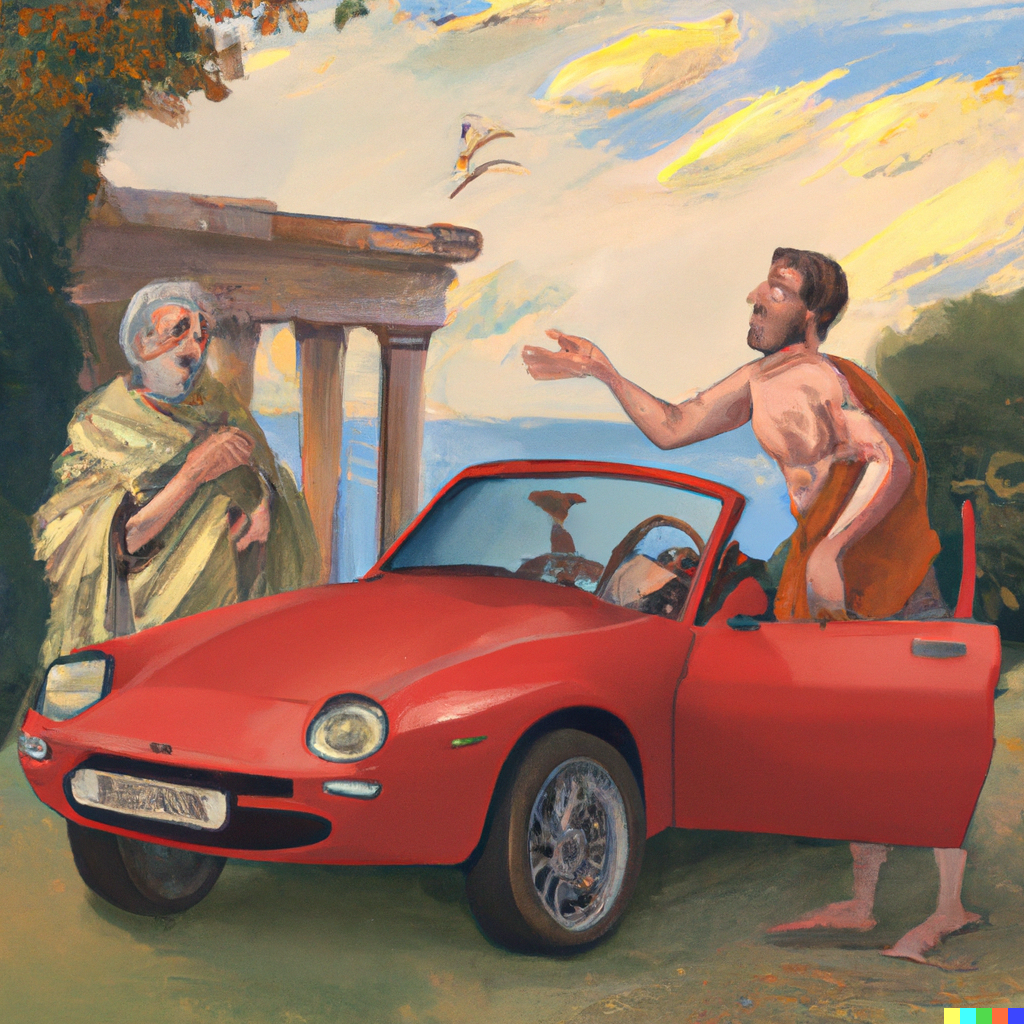
\includegraphics[width=0.5\textwidth]{img/dalle}
\caption{Example of an image generated by DALL-E, when it is asked to generate a painting where Socrates admires Mazda Miata in Ancient Greece.}
\label{img:dalle} 
\end{figure}

Artificial Intelligence can be divided into different types or categories in many ways. Dividing AI into weak or narrow AI and strong AI is a popular high-level way to categorize different Artificial Intelligence methods. In this model, weak AI is AI that is designed to solve specific problems. If the weak AI is given a problem outside the original scope, the weak AI cannot produce reliable results. On the other hand, strong AI is a general-purpose AI that can learn like humans do. Currently, all AI solutions are weak Artificial Intelligences.

Another common high-level way to categorize AI's is to divide them into four different categories; Basic AI, Limited AI, Advanced AI and Superintelligence.

\begin{itemize}
  \item \textbf{Basic AI:} Being the simplest form of AI, the basic AI does not involve any kind of learning. It uses static algorithms, like search algorithms, to produce results.
  \item \textbf{Limited AI:} Limited AI produces results based on a substantial amount of data. Limited AI can learn based on data and produce results by analyzing that data. Machine learning falls into this category.
  \item \textbf{Advanced AI:} Advanced AI has the same intelligence as humans has. Advanced AI can be considered as a general-purpose AI. 
  \item \textbf{Superintelligence:} Superintelligence far surpasses human intelligence.
\end{itemize}

In the context of this thesis, it is perhaps more beneficial to categorize AI based on implementation details. Artificial intelligence solutions have been implemented with different methods throughout the history of AI\cite{russell2010artificial}, such as:

\begin{itemize}
  \item \textbf{Search Algorithms:} Algorithms that can solve many problems by intelligently searching through many possible solutions. Common search algorithms include breadth-first search, depth-first search, A* search, and heuristic-based algorithms. Search algorithms are rarely sufficient for real-world problems, as the number of places to search quickly grows too high.
  \item \textbf{Logic Programming:} AI approach that uses mathematical logic to reason. Rules are specified in the formal logic language.
  \item \textbf{Probabilistic methods for uncertain reasoning:} Probabilistic methods are used to solve the problem when an agent has to act based on uncertain data, using methods from probability theory and economics. Bayesian networks, Markov decision processes, and hidden Markov models are examples of probabilistic methods.
  \item \textbf{Machine Learning:} a subfield of AI that is discussed extensively in this chapter.
  \item \textbf{Artificial Neural Networks (ANNs):} ANNs are models that mimic the functioning of the biological neural networks. ANNs used extensively in deep learning. Examples of artificial neural networks are deep neural networks, convolutional neural networks (CNNs), recurrent neural networks (RNNs), and self-organizing maps (SOMs).
\end{itemize}

\section{Types of Machine Learning} \label{mltypes}

There are four main types of machine learning: supervised learning, unsupervised learning, reinforcement learning and deep learning. Each type has its own characteristics, techniques, and applications. The appropriate type depends on the specific problem, available data, and the desired learning outcome.\cite{burkov2019hundred} 

\subsection{Supervised Machine learning} \label{sml}

The basic idea of Supervised Machine Learning is to predict unknown variables based on known variables. The unknown variable that ML model tries to predict can be a categorical target variable or a numerical target variable. Based on the types of target variables, there are two types of problems in the domain of Supervised Machine Learning; classification problems and regression problems. Training data containing the target variables is called labeled data.

In a classification problem, a supervised ML model tries to predict an unknown category (class label) based on known variables. Classification problems with only two possible outcomes are solved with binary classifiers. This is the case when trying to predict whether a given object is something or not (for example, is this email message spam or not). If there are multiple possible outcomes, then multiclass classifiers are used. In these cases, the model tries to predict the category of a given object (for example, which fruit this fruit is).

In a regression problem, a supervised ML model tries to predict a numerical value for a target variable based on known variables. For example, the model might try to predict the value of real estate based on living area, age, region, etc. of the real estate.

The training dataset consists of instances of data points. Each data point has feature variables (for example, living area, age and region of a real estate) and the target variable (for example, price of the real estate). Data having a target variable called labeled data. When the model is trained, it can be used to predict target variables based on feature variables.

The provided known target variables are what makes supervised machine learning `supervised'.\cite{ml}

\subsection{Unsupervised Machine Learning} \label{usml}

Unlike Supervised Machine Learning, the Unsupervised Machine Learning does not require target variables, so it can operate on unlabeled data. The goal of unsupervised ML is not to predict certain values based on known values, but to find hidden patterns or categorizations in given data.

There is also a type of machine learning that combines techniques from supervised and unsupervised machine learning, called Semi-Supervised Machine Learning.

\subsection{Reinforcement Learning} \label{rl}

Reinforcement Learning learns optimal behaviors through trial and error interactions with an environment. The agent receives feedback in the form of rewards and penalties, and then tries to perform actions that maximize the reward feedback. Reinforcement learning is often used for tasks where an agent learns to take actions to maximize cumulative rewards.

\subsection{Deep Learning} \label{dl}

Deep learning is a complex case of machine learning that uses neural network algorithms to produce results. Neural networks try to mimic the human brain structure. A neural network consists of single nodes or neurons that can communicate with other neurons.

In Deep Learning, the neural networks are aggregated into multiple layers. Each layer extracts more and more higher-level information from the data. Deep learning can use both supervised and unsupervised machine learning.

\section{Machine Learning Algorithms} \label{mlalg}

Machine learning algorithms are mathematical models that are used to perform predictions or decisions based on data. Some of the ML algorithms are specific to the specific type of machine learning, while other ML algorithms can be used in different types of machine learning. Each ML algorithm is suited for different tasks and data characteristics\cite{zhou2021machine}. Examples of ML algorithms:

\begin{itemize}
  \item \textbf{Linear Regression:} A regression algorithm and one of the simplest ML algorithms. Linear regression is used for predicting continuous numerical values based on input variables. It fits a linear relationship between the input variables and the target variable. The example implementation described in Section \ref{implementation} uses linear regression.
  \item \textbf{Logistic Regression:} A classification algorithm that predicts the probability of an instance belonging to a particular class using a logistic function.
  \item \textbf{Decision Trees:} An algorithm that partitions the input into hierarchical decision rules. Decision trees can be used in both regression and classification problems. Algorithms which use multiple decision trees ares called Random Forest algorithms.
  \item \textbf{Support Vector Machines (SVM):} SVM aims to find a hyperplane in an N-dimensional space that classifies the data points. \textit{N} represents the number of features. SVM can be used in both regression and classification problems.
  \item \textbf{K-Nearest Neighbors (KNN):} KNN is used to make predictions based on the similarity of input instances to their neighbors. KNN can be used in both regression and classification problems.
  \item \textbf{Naive Bayes:} An algorithm based on Bayes' theorem that can be used for classification problems.
  \item \textbf{Artificial Neural Networks algorithms:} A class of algorithms that is used with artificial neural networks. ANN algorithms try to mimic the structure of biological neural networks.
  \item \textbf{Clustering Algorithms:} A class of similar algorithms that is used for unsupervised learning. Popular clustering algorithms include K-Means, DBSCAN, and Hierarchical Clustering.
  \item \textbf{Reinforcement Learning Algorithms:}  A class of algorithms that is used with reinforcement learning.
\end{itemize}
\chapter{Trusted Execution Environments} \label{tees}

Trusted Execution Environment (TEE) is a secure environment of a computing device that is isolated from the rest of the system and has its own isolated memory and processing capabilities, preserving confidentiality and integrity. Trusted Execution Environments are not precisely defined, but solutions called TEE's usually have in common that they try to protect the data-in-use, as the more conventional encryption solutions try to protect data-at-rest and data-in-transit. This chapter partly answers to the \ref{rq1}.

Trusted Execution Environments are usually implemented by secure architecture that makes use of hardware features of CPU. TEE's provide a confidential and isolated processing environment, usually backed by hardware-assisted memory encryption.

The idea of TEE's is to provide an isolated environment that is secured from investigation by the rest of the system, allowing development of applications that require high security. For example, TEE's can be used to build systems that allow securing intellectual property, processing of sensitive personal information securely, Digital Rights Management (DRM), secure financial services etc.\cite{teeieee}

As the solution proposed by this thesis is based on Intel's Trusted Execution Environment called Intel Software Guard Extensions (Intel SGX), we focus mainly on that technology, but giving high-level introduction to other TEE platforms.

\section{Use Cases}\label{usecases}

\subsection{Protecting Intellectual Property}\label{protecting1}


With TEE's the decryption and processing of the data can happen completely in a secure environment without the possibility to investigate the data in clear form. This usually requires that the TEE establishes a secure connection for authentication and encryption key exchange outside the environment.

For example, machine learning models can be bundled with application encrypted. The application then decrypts the models only when needed, inside the Trusted Execution Environment.

\subsubsection{Digital Rights Management (DRM)}\label{protecting11}

TEE's provide means for advanced Digital Rights Management. For example, streaming services can protect its content by encrypting the stream data. Encrypted stream data can then be decrypted by the isolated TEE, thus disallowing the customer to copy the content.

\subsection{Protecting Sensitive Personal Information}\label{protecting2}

Sensitive information can be stored encrypted and only decrypted for processing inside the Trusted Execution Environment. This is the case, especially when sensitive information needs to be stored and processed in an untrusted cloud environment.

\subsection{Financial Services}\label{protecting3}

Financial services often have a high security standards. TEE's can help financial services to fulfill these standards by allowing storing and using keys or tokens needed for transactions in an encrypted and isolated environment.

Especially, commerce platforms on mobile devices including Near-Field Communication (NFC) to authorization can benefit from Trusted Execution Environments.

\subsection{Biometric Authentication}\label{protecting4}

The problem with biometric authentication is that the sample of a correct biometric authentication method has to be stored somewhere that then can be compared to input. For example, in a case of fingerprint authentication, the sample of an authorized person's fingerprint needs to be stored in some form. When the sample is stored unprotected, it is possible to retrieve it and use it for authentication.

With TEE's the sample can be stored encrypted and the comparing process can then happen completely in the isolated environment, where the sample is decrypted, thus disallowing any investigation of the sample by the outside world.

\section{Intel Software Guard Extensions (Intel SGX)}\label{sgx}

Intel introduced new security-related instruction codes called Security Guard Extensions (SGX) in 2015 part of the sixth generation Intel Core processor family release. At the time of writing this thesis (2023), Intel has dropped support for SGX in consumer CPU model Intel Core, but continues development on the enterprise Intel Xeon series of processors.

Software Guard Extensions allow user- or operating system -level code to create hardware-backed secure and isolated processing environments, called Enclaves. Enclaves are in a specific isolated and encrypted part of the memory and content is decrypted on the fly inside the CPU when processing.

Code inside the enclave cannot be examined by the rest of the system by any code that is running with higher privileges, not even by computer firmware or hypervisors in a virtual environment.

In the Intel SGX application, the application code is divided into trusted and untrusted parts. The untrusted part handles the creation of the enclave and communication with the rest of the system. The trusted part runs inside the enclave. Usually, most of the application code is in the untrusted part, as it is recommended to operate inside the enclave only when it is really necessary, due to the limited memory of the enclave.\cite{mit}

Intel SGX has some vulnerabilities, most of them based on the side-channel attack.\cite{sgxfail}

\subsection{Remote Attestation}\label{remoteattestation}

Remote attestation is an Intel SGX feature that enables trust between a remote server and the application running in the Intel SGX enclave. The remote server can verify that the application is, in fact, running in the fully working SGX enclave and all the latest security patches are applied.

The main use case of remote attestation is to verify that it is safe to open up the secure channel between the remote server and the application running in the enclave. After the remote attestation is complete, information can be exchanged safely through the secure channel.

Intel provides two different methods for remote attestation. Enhanced Privacy ID (Intel EPID) based attestation method can be used on older Intel SGX capable processors that do not support Flexible Launch Control. This attestation method requires usage of Intel's attestation service.

Elliptic Curve Digital Signature Algorithm (ECDSA) Attestation is the second of the attestation methods. This method requires newer processor models that support Flexible Launch Control. On the other hand, the attestation service can be self-hosted.

\subsection{Using Intel SGX on Linux}\label{usingsgxonlinux}

Running Intel SGX applications on Linux requires two software parts to be installed: Intel SGX driver and Intel SGX Platform Software (PSW). 
To be able to build Intel SGX applications, also the Intel SGX Software Development Kit (SDK) needs to be installed. Of course, the Intel SGX support needs to be enabled on the hardware level (BIOS/UEFI) too. Intel provides repositories for software required for the supported Linux distributions.

Currently, Intel supports the next Linux distributions: Red Hat Enterprise Linux, CentOS Server, Ubuntu Server, SUSE Linux Enterprise Server, Anolis OS, Debian.

The Linux kernel supports Intel SGX natively from kernel version 5.11, but only processor models with Flexible Launch Control support. If the processor does not support Flexible Launch Control, the Out-of-Tree (OOT) driver and kernel version lower than 5.11 must be used.

To check that the Intel SGX support is enabled, \textit{cpuid} utility could be used. Example lines from \textit{cpuid} output showing Intel SGX support in Listing \ref{alg:cpuid}.

\begin{algorithm}
\begin{minted}{text}
  Software Guard Extensions (SGX) capability (0x12/0):
      SGX1 supported                           = true
      SGX2 supported                           = false
\end{minted}
\caption{Example cpuid output for discovering Intel SGX support.\label{alg:cpuid}}
\end{algorithm}

Intel has provided very detailed installation instructions for all the software parts needed for different platforms and processor models.\cite{sgxinstall} The Intel SGX SDK has a directory \textit{SampleCode} which contains multiple C++ application and build configuration examples.

\subsection{Limitations}\label{limitations}

The additional security provided by Intel SGX does not come free of limitations. The most obvious limitation is that the hardware must be chosen from Intel processors that have Intel SGX support. Running applications inside an Intel SGX enclave has limited performance. From the perspective of a processor-heavy machine learning calculations, the limited performance might be an issue. The performance degradation is discussed in detail in the Section \ref{performance}.

Another limitation is that the enclave size is limited by the maximum amount of memory that an enclave can allocate. The maximum memory amount that can be allocated is determined mainly by the Enclave Page Cache (EPC) size that is usually between 64 MB and 256 MB and depends on the processor model and firmware. On Linux, the EPC size limit can be bypassed by EPC swapping, but that adds additional performance overhead. \cite{graminedocs}

On the modern Intel Xeon server processors, starting with Ice Lake models, the EPC size can be up to 1 TB. With the 1 TB limit, the size of an enclave does not be an issue in most cases.

The EPC size can be discovered by Gramine\cite{gramine} utility \textit{is-sgx-available}. Example output can be seen in Listing \ref{alg:issgx}. The example output reports the EPC size to be 5d80000 bytes in hexadecimal, which is 98041856 bytes (98 MB) in decimal. 

The limitations of the development process of an Intel SGX application must also be considered. Intel SGX applications must be written in C or C++ and they must follow specific structure. Intel SGX does not allow dynamic linking, so libraries must be statically linked to the application. Many popular machine learning libraries for C++ do not offer a statically linked version of the library.\cite{sgxdev}

The development process restrictions can be eased with frameworks like Gramine\cite{gramine} which can wrap, for example, applications written in Python in Intel SGX compatible application. Gramine is discussed in more detail in the next section.

\begin{algorithm}
\begin{minted}{text}
...
Max enclave size (32-bit): 0x80000000
Max enclave size (64-bit): 0x1000000000
EPC size: 0x5d80000
SGX driver loaded: true
...
\end{minted}
\caption{Example is-sgx-available output for discovering EPC size.\label{alg:issgx}}
\end{algorithm}

\subsection{Gramine LibOS}\label{gramine}

Gramine is a lightweight Library Operating System (LibOS) which allows single applications to be run isolated with a minimal operating system. Gramine was first developed in OSCAR LAB at Stony Brook University, but many contributors joined the development process, including Intel Research Lab, which contributed to the Intel SGX support. 

Library operating system can be compared to running a full operating system inside a virtual machine, but much more lightweight and minimalistic approach.

Gramine allows applications to be run inside the Intel SGX enclave without the need to port them to Intel SGX C or C++ applications. Even applications written in interpreted languages, like Python, can be run inside enclave. Gramine enables this by wrapping the application code with interpreter and needed libraries inside a Gramine application, which can be then run inside the Intel SGX enclave.\cite{graminedocs}

The Gramine LibOS itself adds a memory cost just of 5 to 15 MB, but when running Gramine application inside Intel SGX enclave, other performance implications appear. In the paper\cite{graminesgxwp} by the Gramine team from 2017, the performance effects of running simple operations inside the Intel SGX enclave were discussed. Based on the measurements that Gramine team has conducted, running simple operations inside an enclave were approximately 100\% slower than locally, as can be seen in Figure \ref{img:graminebenchmark}. The more memory intensive the operation was, the more overhead it adds.

\begin{figure}
\centering 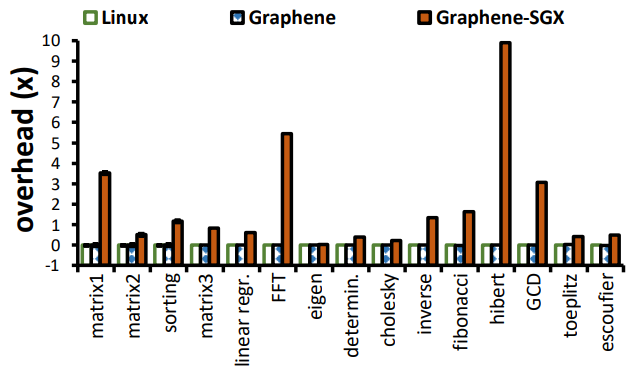
\includegraphics[width=0.7\textwidth]{img/graminebenchmark}
\caption{Performance overhead of Graphene-SGX, presented in \textit{Graphene-SGX: A Practical Library {OS} for Unmodified Applications on SGX}}
\label{img:graminebenchmark} 
\end{figure}

Gramine applications are configured in a special manifest file which uses TOML syntax. Configurable values include application entry point, enclave settings, remote attestation settings and trusted files. A part of a manifest file from the implementation that is provided as a part of this thesis can be seen in Listing \ref{alg:graminetoml}.

\begin{algorithm}
\begin{minted}{toml}
sgx.trusted_files = [
    ...
    "file:trusted.py",
    "file:ca.crt",
    "file:model_encrypted",
    "file:cars.csv",
]
\end{minted}
\caption{Part of Gramine application manifest file defining trusted files\label{alg:graminetoml}}
\end{algorithm}

Installation and usage of Gramine is discussed in the Chapter \ref{solution}. In the Section \ref{performance}, it can be seen how measurements conducted in this thesis aligns with the measurements conducted by Gramine team.

\section{AMD Secure Encrypted Virtualization (SEV)} \label{sev}

AMD's Secure Encrypted Virtualization (SEV) is a hardware-backed Trusted Execution Environment platform that allows an encryption of a virtual machine memory. AMD SEV is supported on AMD EPYC server processors. AMD SEV requires usage of the Linux built-in hypervisor Kernel-based Virtual Machine (KVM).

AMD SEV has no need for code changes to the application, as the whole memory used by the virtual machine is encrypted. There are also no memory limits other than physical memory. On the other hand, security features are limited compared to the Intel SGX.\cite{suse}

\section{ARM TrustZone} \label{trustzone}

ARM TrustZone is the oldest and the most used Trusted Execution Environment platform mentioned in this thesis. AMD TrustZone is a hardware-backed TEE supported on ARM Cortex-A and ARM Cortex-M microcontrollers, first introduced in 2004. There are some differing infrastructure details between the implementation of the Cortex-A and Cortex-M microcontroller families. The main usage platform is mobile devices, and some of the mobile device manufactures use ARM TrustZone comprehensively.\cite{trustzone}

\section{Cloud Provider's Solutions} \label{cloudprovider}

Amazon Web Services (AWS), Google Cloud Platforms (GCP) and Microsoft Azure all offer Trusted Execution Environment implementation on their cloud computing platforms. They are rather novel technologies, and low-level implementation details are not publicly available for all of them.

\subsubsection{Amazon Web Services} \label{aws}

Amazon Web Services offers AWS Nitro Enclaves that allows users to convert an application to a special Enclave Image File (EIF) that can be used to launch an enclave. AWS Nitro Enclaves are hardware-agonistic and the implementation is published as open source.\cite{aws}

\subsubsection{Google Cloud Platform} \label{gcp}

Google Cloud Platform offers multiple different TEE solutions, some of them based on AMD's Secure Encrypted Virtualization. Computing units, for example virtual machines or GKE nodes, can be launched in a confidential environment backed by AMD SEV.\cite{gcp}

\subsubsection{Microsoft Azure} \label{azure}

Microsoft Azure offers confidential computing by supporting both Intel SGX and AMD SEV on their platform. Microsoft Azure also offers surrounding TEE-related infrastructure to make TEE operations more convenient, for example, Microsoft Azure Attestation that allows attestation of multiple Trusted Execution Environments at once.\cite{azure}

\chapter{Solution} \label{solution}

The solution proposed in this thesis uses an approach where the distributed application is bundled with an encrypted ML model. To be able to decrypt the encrypted ML model, the distributed application opens a secure channel to the special, remote attestation capable key server. After the key server has validated that the application runs in a secure and isolated environment -- an enclave, and the application has not been tampered with, the key server transfers the decryption key to the application. The encrypted ML model is then decrypted inside an enclave and only used within the enclave, and never exposed outside the enclave.

Using this approach, the confidentiality and integrity of the ML application is not compromised, and the intellectual property associated with the ML model is safe. The solution proposed in this thesis is demonstrated by implementation described in the next section.

By providing a practical solution to the concern regarding the safety of the IP associated with ML models, this chapter answers to the \ref{rq2}. Later in this chapter, in Section \ref{perfandlimitations}, the issues, limitations and effects on performance are discussed, thus answering to the \ref{rq3}.

\section{Implementation} \label{implementation}

The example implementation consists of three parts; the model trainer, the key server and the distributed application itself, called predictor, which will be discussed in detail later. The model trainer trains the ML model and exports it to an encrypted file with a decryption key. The key server acts as a remote attestation capable key server from which the predictor can request a decryption key. The predictor part is the application that can be distributed to the clients. In this implementation example, the predictor is an application that predicts car fuel consumption based on user inputted details.

The predictor is bundled with an encrypted machine learning model and Gramine Python application, which runs inside Intel SGX enclave. The Gramine application has a machine learning framework bundled and utilities to request remote attestation and decryption key from the key server through a secure channel. The key server uses Intel SGX Remote Attestation to validate the enclave before providing the decryption key. Because of the key exchange and remote attestation, minimal internet connection is required in the production environment. The high-level application flow can be seen in Figure \ref{fig:sgx-flow}.

The predictor part is further divided into two parts, trusted (\textit{trusted.py}) and untrusted (\textit{predictor.py}). The trusted part (Gramine application) runs inside the Intel SGX enclave and has only the minimal needed functionality in addition to the Intel SGX related functionality. Additional capabilities are the capability to decrypt the ML model and the capability to run ML calculations on that model. The untrusted part has all the other application logic and calls the trusted part only when it is needed to do ML calculations.

\begin{figure}
\centering 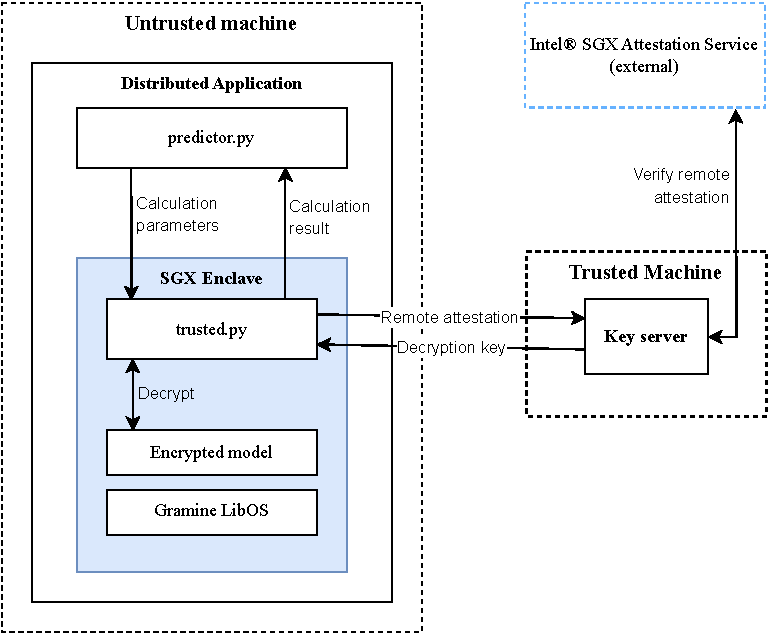
\includegraphics[width=0.8\textwidth]{img/sgx}
\caption{Application flow diagram}
\label{fig:sgx-flow}
\end{figure}

 Python was chosen as the main implementation language as Python has great machine learning tool support. Intel SGX was chosen as Trusted Execution Environment implementation. Running Python inside the SGX enclave is possible using the library operating system Gramine.\cite{gramine} Running Python inside the enclave is already demonstrated by Denghui Zhang, Guosai Wang, Wei Xu and Kevin Gao in their paper \textit{SGXPy: Protecting Integrity of Python Applications with Intel SGX}\cite{sgxpy}.

The model trainer and the key server are intended to run on the trusted infrastructure and do not require hardware Intel SGX support. Both model trainer and key server are needed to build artifacts for the distributed application. Artifacts includes key server certificate generated when the key server is built and the encrypted ML model generated by the model trainer. Furthermore, the key server needs access to the decryption key generated by the model trainer. The predictor which uses the ML model for computation is run in an untrusted environment. 

As the ML model is bundled encrypted with the predictor application and only processed decrypted inside the Intel SGX enclave, the Intellectual Property of the model owner is safe.

There is a repository containing all the software source code at GitHub\cite{githubrepo}.

\subsection{Description of the Data} \label{data}

The dataset used to train the machine learning model contains 398 instances of cars with 8 attributes. The attributes are miles per gallon (MPG), cylinders, engine displacement in cubical inches, horsepower, weight in pounds, acceleration ($ft/s^2$), year of making, origin and name of the model. Origin is marked as an integer, where 1 means United States, 2 means Europe and 3 means Japan.

The dataset is from the Machine Learning Repository by University of California, Irvine\cite{dataset}. The data is in CSV format. Example data points can be seen in Table \ref{tab:data}.

\begin{table}
\centering{}\caption{Example data points of the dataset.\label{tab:data}}
\begin{tabular}{|c|c|c|c|c|c|c|c|c|}
mpg & cyl. & displ. & hp & weight & accel. & year & origin & name \tabularnewline
\hline 
23.7 & 3 & 70.00 & 100.0 & 2420 & 12.5 & 80 & 3 & Mazda RX-7 \tabularnewline
19.0 & 6 & 156.0 & 108.0 & 2930 & 15.5 & 76 & 3 & Toyota Mark II \tabularnewline
11.0 & 8 & 400.0 & 150.0 & 4997 & 14.0 & 73 & 1 & Chevrolet Impala \tabularnewline
\end{tabular}
\end{table}

\subsection{Overview of the Application Stack} \label{overview}

\subsubsection{Model Trainer} \label{modeltrainer}

The model trainer is part of the implementation that is responsible for training the machine learning model and exporting it as an encrypted file with a decryption key. The model trainer is meant to run in a trusted environment as a part of the build process.

The original dataset needed to be cleaned for empty values and inconsistent formatting. The dataset was split into two datasets, \textit{cars1.csv} which has 242 data points (16 KB) and \textit{cars2.csv} which has 150 data points (8 KB). The \textit{cars1.csv} was used to train the model and \textit{cars2.csv} was used to test the model. Except for the car model name, all other data attributes were used to train the model.
 
As a machine learning library, the Python library \textit{Scikit-learn}\cite{scikit} was used. Linear Regression is used as an ML algorithm to train the model. Other Python libraries used were \textit{Cryptography} for cryptographic functions and \textit{Pandas} for easy CSV handling.

As the original dataset has only 398 data points, a synthetic data generator was also implemented as a part of the model trainer. Synthetic data is used in later sections to run performance testing on large datasets.

Model trainer is used in the application build process, where the model is trained, encrypted and exported to the application bundle and the decryption key is exported to the key server. The exported model is 4 KB in size.

\subsubsection{Key Server} \label{keyserver}

The key server is used to securely provide the decryption key for the predictor application. The security of the decryption key transfer is confirmed by Intel's Remote Attestation. Remote attestation confirms that the application code is running inside an enclave and the application is not tampered with. Using remote attestation makes sure that the decryption key (and decrypted ML model) is only handled inside an enclave, and it is impossible for the application user to obtain the key or the decrypted model. The key server is meant to run in a trusted environment.

The key server is a C application based on Intel's example code. The key server acts as an HTTPS server from which the application can request the decryption key. When the application requests for the key, the Remote Attestation is performed and if it is successful, the key server returns the decryption key.

\subsubsection{Predictor} \label{predictor}

The predictor application is the main application which is meant to be distributed to the end user and run inside an untrusted environment. The application predicts fuel consumption of a car based on the car's other attributes that are inputted by the end user. There are also options for running the predictions for a predefined dataset or running predictions locally, outside the Intel SGX enclave. These additional options are mainly for performance testing purposes.

The predictor application follows Intel SGX application structure and has two parts; untrusted and trusted. The untrusted part (\textit{implementation/predictor/predictor.py} in the GitHub repository) has all the application logic and calls the trusted part only for the ML calculations. Executing the untrusted part starts the predictor application and is meant to be called directly by the end user. Trusted part (\textit{implementation/predictor/trusted/trusted.py} in the GitHub repository) is the part of the application that is responsible for handling all the sensitive tasks. Sensitive tasks are the handling of the decryption key and decrypted ML model.

An encrypted machine learning model is bundled with the predictor application. Model is handled in plain only inside the trusted part, and it is impossible to decrypt it outside the trusted part.

When the application is started by invoking the untrusted part, it asks the user for the car details. After the details are filled in, the trusted part is invoked by the untrusted part and the car details are sent to the trusted part.

When the trusted part is invoked, the Intel SGX enclave is created and initialized, remote attestation is requested from the key server, and after successful remote attestation, the decryption key is received from the key server. Now the encrypted ML model that is bundled with the application is decrypted, and the ML calculations are performed, all inside the trusted part.

After the ML calculations are ready, the results returned to the untrusted part, which formats them and presents to the user. Results include the predicted fuel consumption, running time, data point count and, in a case of running predictions on a dataset, the R2 score, which is a calculated metric describing the accuracy of the ML model.

The application has a simple command line interface for interacting with the user. Trusted and untrusted part communicate with each other with a simple interface, which was implemented. The interface for inter-application communication used command line parameters to send data to the trusted part and standard output to receive results from the trusted part. The data format is JSON. An example of the communication between the untrusted and the trusted part can be seen in Listing \ref{alg:communication}.

In a production-ready application, the inter-application communication interface should be more sophisticated. For example, running an HTTP server inside an enclave is possible.

\begin{algorithm}
\begin{minted}{python}
# To trusted part
{'cylinders': [4], 'displacement': [97.5], 'horsepower': [114.0],
'weight': [2094], 'acceleration': [10.5], 'year': [90], 'origin': [3]}

# From trusted part
{'predictions': [39.557013442440216], 'time': 0.004551887512207031,
'count': 1, 'r2': null}
\end{minted}
\caption{An example of inter-application communication.\label{alg:communication}}
\end{algorithm}

\subsection{Setting Up} \label{settingup}

Next, the requirements and prerequisites which are needed to build the application and the build of the application are discussed in detail.

\subsubsection{Requirements} \label{requirements}

The model trainer can be run anywhere where there is Python available and enough resources to train a simple machine learning model.

The key server needs working Gramine installation with remote attestation support. Hardware Intel SGX support is not needed.

The predictor application needs an environment that supports Intel SGX. Section \ref{usingsgxonlinux} and \textit{Intel® SGX Software Installation Guide For Linux* OS}\cite{sgxinstall} can be referred for detailed instructions. Gramine documentation\cite{graminedocs} can be referred for Gramine installation instructions.

The next Python libraries need to be installed system-wide. The easiest way is to install them is to install them from the distribution package repositories.

\begin{itemize}
  \item \textit{scikit-learn} as a machine learning framework.
  \item \textit{cryptography} for cryptographic functions.
  \item \textit{pandas} for handling CSV's.
  \item \textit{joblib} for exporting and importing ML models.
\end{itemize}

\subsubsection{Remote Attestation} \label{remoteatt}

The implementation uses the \textit{Intel SGX Attestation Service Utilizing Enhanced Privacy ID (EPID)} method for remote attestation. Developer access for Intel EPID can be requested from the Intel Trusted Services Portal.\cite{intelportal} This implementation requires unlinkable EPID subscription, which is free for non-commercial use.

The SPID identifier and EPID API key can be acquired from Intel Trusted Services Portal after subscription.

\subsubsection{Build} \label{build}

After the Intel SGX support, Gramine and other dependencies are installed, the application itself can be built. The application code can be downloaded from \url{https://github.com/mjturt/thesis}. In the application's implementation folder, the example settings file \textit{settings.sh-example} needs to be copied to \textit{settings.sh}. At least two configuration parameters need to be configured in the settings file. Configuration parameters \mintinline{bash}{RA_CLIENT_SPID} and \mintinline{bash}{RA_TLS_EPID_API_KEY} represents SPID identifier and EPID API key, which were obtained from Intel Trusted Services Portal in the last section.

In the implementation folder, there is a \textit{build.sh} script to automate the build process. The build script initiates the model trainer, which trains the ML model with data from file \textit{implementation/model-trainer/data/cars1.csv}. When the model is trained, the model trainer encrypts it and exports the encrypted model and the decryption key to files. The build script then makes the encrypted model available to the predictor and the decryption key available to the key server. After that, the key server is compiled and built. The key server exports the needed SSL certificate as a part of the build process, and the build script makes it available to the predictor.

Next, the build script instructs the user how the predictor can be built and how to launch the application. When the predictor is built based on these instructions, the application stack can be launched, which will be covered in the next section. An example installation process can be seen in Listing \ref{alg:install} and a diagram of the build flow can be seen in Figure \ref{fig:sgx-build}.

\begin{figure}
\centering 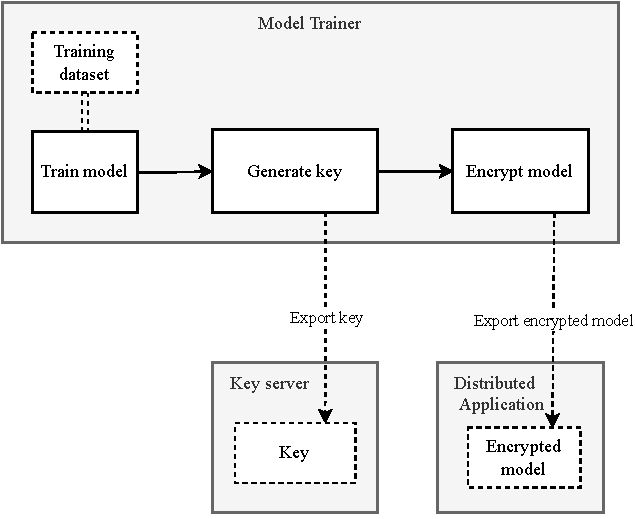
\includegraphics[width=0.8\textwidth]{img/sgx_build}
\caption{Build flow}
\label{fig:sgx-build}
\end{figure}

In a real-life scenario, the predictor could now be packed and distributed to the end-users, but for simplicity, the whole application stack is run on the same machine.

\begin{algorithm}
\begin{minted}{bash}
git clone https://github.com/mjturt/thesis.git
cd thesis/implementation
cp settings.sh-example settings.sh  # and configure
source settings.sh
./build.sh
cd predictor/trusted
make SGX=1
\end{minted}
\caption{Installation procedure of the application.\label{alg:install}}
\end{algorithm}

\subsection{Usage} \label{usage}

After installation is complete, the key server can be started in the \textit{implementation/key-server} folder by running \mintinline{bash}{./server_epid}. The key server is left running. Now the setting up is complete, another shell session needs to be opened, and then the predictor can be executed in the \textit{implementation/predictor} folder by running \mintinline{bash}{python predictor.py}. The settings file \textit{settings.sh} must always be sourced in the shell session from where the key server or predictor is invoked.

\begin{algorithm}
\begin{minted}{text}
...
For a car:

Model: Mazda MX-5
Cylinders: 4
Displacement: 97.5 in³ (1597.7 cm³)
Power: 114.0 hp (85.0 kW)
Weight: 2094.0 lb (950.0 kg)
Acceleration: 10.5 ft/s² (3.2 m/s²)
Year: 1990
Origin: Japan
Predicted consumption: 39.6 mpg (5.9 l/100km)

The predicted consumption is 5.9 l/100km
The prediction calculation took 0.004552 seconds
\end{minted}
\caption{Output of the predictor application without any parameters.\label{alg:output}}
\end{algorithm}

\begin{algorithm}
\begin{minted}{text}
Sending dataset cars.csv to the Gramine Intel SGX enclave for
calculation...

--- START OF GRAMINE OUTPUT ---
...
--- END OF GRAMINE OUTPUT ---

Consumption prediction calculation for 150 car instances took
0.002998 seconds
R2 score: 0.81
\end{minted}
\caption{Output of the predictor application using a dataset.\label{alg:output2}}
\end{algorithm}

Without any parameters, the predictor application \textit{predictor.py} asks the user for the car details and then runs ML calculations inside an enclave. The predictor can be invoked with a command line argument \mintinline{bash}{--help} to get all available command line argument options. Available command line arguments include an argument to run predictions on a predefined dataset and an argument to disable Intel SGX. An example output of the predictor without any parameters and after it has asked the car details can be seen in Listing \ref{alg:output}. Non-relevant output has been omitted.

An example output of the predictor using a predefined dataset can be seen in Listing \ref{alg:output2}. In this listing, only the Gramine output is omitted.

\section{Performance and Limitations} \label{perfandlimitations}

In this section, the testing setup used to conduct performance testing is described, including the hardware and software used. The performance testing research setting is described, and the performance testing results are then presented, and perceived limitations and downsides are discussed. The general limitations of Intel SGX can be read from Section \ref{limitations}.

\subsection{Testing Setup} \label{setup}

For the simplicity sake, in the testing setup, the model trainer, the key server and the distributed app are built and run on the same machine.

As a testing hardware, Dell Latitude 5490 laptop provided by the University is used. The laptop has an 8th generation Intel Core i5 processor that has Intel SGX support. The specifications of the testing hardware and software below:

\begin{itemize}
  \item \textbf{OS:} Ubuntu Server 22.10 
  \item \textbf{Kernel:} Linux 5.10.15
  \item \textbf{CPU:} Intel Core i5-8350U 8-core 3.6 GHz (code name Kaby Lake R)
  \item \textbf{Memory:} 16 GB
\end{itemize}

The processor did not have Flexible Launch Control (Intel SGX Launch Control) support, so the Linux in-kernel SGX driver could not be used, as the in-kernel driver requires it. Out-of-tree (OOT) driver was used instead.

As an operating system, Ubuntu Linux 22.10 was used. As of the time of writing, Ubuntu 22.10 used kernel version 5.19 that has the in-kernel SGX driver that is incompatible with the out-of-tree SGX driver. The Linux kernel version had to be downgraded to version 5.10.

After downgrading the kernel, the Intel's official documentation\cite{sgxinstall} to install out-of-tree SGX driver was followed.

Next, the Gramine library OS can be installed. Because of the OOT driver, Gramine needed to be built from source. Gramine documentation\cite{graminedocs} was followed to build Gramine from source with custom options.

All needed Python libraries were installed system-wide from the default Ubuntu APT repositories.

As the processor model is older than the Ice Lake series, the EPC size is limited to 98 MB. With enclaves that require more than that, there would be substantial performance degradation. As the Intel SGX OOT driver does not support EPC swapping, testing with enclaves larger than 98 MB could not be performed.

\subsection{Performance} \label{performance}

As Machine Learning calculations can be expensive, the overhead produced by running the calculations inside the Intel SGX enclave must be carefully considered. The usability of this solution depends on how much Intel SGX adds overhead.

In the testing setup, a dataset with 150 data points and a dataset with one million data points representing cars were used. The dataset with 150 data points was from the original dataset (file \textit{implementation/model-trainer/data/cars2.csv} in the repository), and the dataset with one million data points was generated with the model trainer's data generation utility. Running inference for data points ran as a batch and total time was recorded. The predictor application has an option to run inference inside Intel SGX enclave or locally. The two methods to run inference are then compared.

\begin{algorithm}
\begin{minted}{python}
test_X, test_y = build_data(data)
start = time()
result = model.predict(test_X)
end = time()
elapsed_time = end - start
\end{minted}
\caption{Python code to run inference and measure time elapsed.\label{alg:time}}
\end{algorithm}

Only the run time of the actual inference is recorded, as can be seen in Listing \ref{alg:time}. Other performance implications to the process are reviewed separately.

For both methods and both datasets, 5 runs conducted and then an average of running time is calculated. Running times for 150 data point inference can be seen in Table \ref{tab:performance} and running times for one million data point inference can be seen in Table \ref{tab:performance2}.

The dataset with 150 data points was 4 KB in size and the dataset with one million data points was 44 MB in size, so the EPC size limit did not affect the measurements.

Based on performance testing, running inference inside the Intel SGX enclave is considerably slower than without the Intel SGX enclave, based on the dataset size. With the smaller dataset, the inference inside SGX enclave is only approximately two times slower, but when a dataset grows to one million data points, the inference inside SGX enclave is approximately thirty-three times slower. It seems that the bigger the dataset is, the more the Intel SGX is lowering the performance.

\begin{table}
\centering{}\caption{Run times of 150 data point inference with both methods.\label{tab:performance}}
\begin{tabular}{|c|c|c|}
Run & Intel SGX & Local \tabularnewline
\hline 
1 & 2.75 ms & 0.97 ms \tabularnewline
2 & 3.01 ms & 0.99 ms \tabularnewline
3 & 2.73 ms & 0.96 ms \tabularnewline
4 & 3.05 ms & 0.99 ms \tabularnewline
5 & 3.20 ms & 0.97 ms \tabularnewline
\hline 
\textbf{Average} & \textbf{2.95 ms} & \textbf{0.98 ms} \tabularnewline
\end{tabular}
\end{table}

\begin{table}
\centering{}\caption{Run times of million data point inference with both methods.\label{tab:performance2}}
\begin{tabular}{|c|c|c|}
Run & Intel SGX & Local \tabularnewline
\hline 
1 & 782.19 ms & 23.15 ms \tabularnewline
2 & 784.03 ms & 23.35 ms \tabularnewline
3 & 787.77 ms & 24.04 ms \tabularnewline
4 & 791.85 ms & 23.19 ms \tabularnewline
5 & 792.61 ms & 23.88 ms \tabularnewline
\hline 
\textbf{Average} & \textbf{787.69 ms} & \textbf{23.52 ms} \tabularnewline
\end{tabular}
\end{table}

Besides the actual running time, the initialization of the Intel SGX application needs to be considered. Initialization of the Gramine, the enclave and performing Remote Attestation takes up to one minute on the testing machine. In the testing setup, the application and the key server run on the same machine, so network latency can increase the initialization in production environment. In any case, the Intel SGX application is usually kept running and initialization does not happen every time when interacting with the application.

\subsection{Limitations and Drawbacks} \label{perceivedlimitations}

One of the most obvious limitations is the EPC size limit of 98 MB in the testing setup. On the testing machine, it is impossible to run enclaves bigger than the EPC size. When tried to run inference for a dataset with 3 million data points (130 MB), the application simply fails because not enough memory could be allocated. However, the EPC size limit is an issue only with older Intel hardware.

In a scenario where the ML application is distributed to the end-users, the hardware and software requirements that end-users must meet, might become a major limitation. End-users infrastructure must fully support Intel SGX, which may make this solution unappealing to some potential customers. One possible solution to this problem is that the ML application is provided as an end-to-end solution, where infrastructure and support is included in the product. This obviously increases the cost of the solution.

The major downside of the approach of using Intel SGX to protect ML models is the engineering overhead it adds. Hardware and software must be carefully chosen, so that the full potential of Intel SGX can be reached. Configuring the system to fully support Intel SGX is a complex operation which requires understanding of the hardware and operating system used. Building Intel SGX applications is more complex than building just regular applications, though frameworks like Gramine can help the process.

\chapter{Conclusion} \label{conclusion}

This thesis has explored the potential of trusted execution environments, especially Intel SGX, in protecting intellectual property of machine learning models. The rapid growth of the AI industry has raised concerns about the safety of the ML model intellectual property. The risen concerns have led to an increased demand for more efficient methods to protect the ML models from tampering and theft. The existing methods used to protect intellectual property of a software, such as data obfuscation and legal protection, have proven to be insufficient in a case of a machine learning application.

Trusted execution environments have emerged as a promising solution to the concern regarding intellectual property of the ML models. Intel's Software Guard Extension is one of the most popular TEE implementations. This thesis has explored the suitability, benefits, limitations and drawbacks of using Intel SGX to provide a secure environment where the data of the ML model would be safe, especially in a case where machine learning application is distributed to the end-users with the ML model bundled with it.

At the beginning of this thesis, different scenarios where security of the ML model is questioned, were described, following with an introduction to artificial intelligence and machine learning. Next, trusted execution environments were discussed in more detail, which answers to the \ref{rq1}. Possible use cases of TEEs and different TEE implementations were explored. The main focus was on Intel SGX, and its general limitations were described.

This thesis shows that Intel SGX can effectively be used to protect intellectual property of the ML models, with certain limitations. This thesis proposes a solution where ML model is bundled with the application encrypted. After Intel's remote attestation feature is used to confirm that the application is run inside a secure and isolated enclave and the application has not been tampered with, a decryption key is provided for the application through a secure channel. The decryption of the ML model happens inside an enclave, and it is used unencrypted only inside an enclave, thus ensuring confidentiality and integrity of the ML model. The intellectual property of the ML model is secure as it is not exposed outside an enclave in any way. The proposed solution answers to the \ref{rq2}.

However, it is important to acknowledge that the solution proposed does not come without limitations. This thesis shows that the implications on the performance are considerable. Based on measurements that were conducted in this thesis, running machine learning calculations inside Intel SGX enclave are two to thirty-three times slower than running the same calculations locally. Based on measurements, the more data is provided for the ML model, the higher the performance implications were. Machine learning calculations can be expensive, and the performance implications needs to be considered when considering the solution's suitability.

There were also other limitations or drawbacks to the solution. On older Intel hardware, the enclave size is limited. All the data that is processed, the application and the ML model needs to fit inside the enclave, so this can be a considerable limitation. Also, the additional engineering work that is needed to design and build a machine learning application that is run inside an enclave is considerable, compared to just designing and building a regular machine learning application. The cost of engineering overhead might make this solution unappealing in some cases. The description of the discovered limitations and drawbacks answers to the \ref{rq3}.

This thesis provides an example implementation which further demonstrates the suitability and limitations of the solution proposed. The example implementation is used to conduct performance measurements.

% The thesis main content ends here.

\printbibliography

\end{document}
